\documentclass{beamer}

\usepackage[utf8x]{inputenc}
\usepackage{default}
\usetheme{PaloAlto}
\usecolortheme{seahorse}

\title{Sistemas Digitais 2\\ \textbf{Projeto de Circuitos Sequenciais}}
\date{\today}
\institute{\textbf{Universidade de Brasília - Faculdade do Gama}} 

\begin{document}

%SLIDE INICIAL DE APRESENTAÇÃO
\begin{frame}
  \titlepage
\end{frame}
  
%SLIDES == INTRODUÇÃO
\section{Introdução}
\begin{frame}
  \frametitle{Introdução}
  \begin{itemize}
   \item Quando realizamos a análise de um circuito, queremos obter a descrição do mesmo. \pause
   \item Se quisermos construir o circuito, o que devemos fazer? \pause
   \item Para construir o circuito fazemos praticamente o contrário da análise.
  \end{itemize}
\end{frame}

\begin{frame}
 \frametitle{Introdução}
 O processo de projetar um circuito sequência pode ser dividido em sete etapas, são elas:
 \begin{block}{Etapas}
  \begin{enumerate}
   \item Partindo da descrição do circuito produza o diagrama de estados.\pause
   \item Derive a tabela de próximo estado do diagrama de estados.\pause
   \item Converta a tabela de próximo estado em uma tabela de implementação.\pause
   \item Derive as equações de excitação para cada entrada de flip-flop da tabela de implementação.\pause
   \item Derive a tabela de saída do diagrama de estados.\pause
   \item Derive as equações de saída da tabela de saída. \pause
   \item Desenhe o diagrama do circuito baseado nas equações de excitação e saída.
  \end{enumerate}

 \end{block}

\end{frame}


%SLIDES == EXEMPLO
\section{Exemplo}
\begin{frame}
  \frametitle{Exemplo}
  Desenvolvemos um exercício no qual aplicamos estes passos.\pause
  
   \begin{block}{Exemplo}
    \begin{center}
    Projete um circuito sequencial que conte a seguinte sequencia: \\3, 7, 2, 6, 3, 7, 2, 6 … \\ Teremos uma entrada C que inicializa ou termina o circuito. 
    Todos os estados não utilizados devem ser levados ao estado inicial, ou seja, o estado 3. Utilizar FF D e representar a contagem diretamente dos FF.
    \end{center}
   \end{block}
\end{frame}

%SLIDES == EXEMPLO DIAGRAMA DE ESTADOS
\begin{frame}
  \frametitle{Exemplo(Diagrama de estados)}
  \begin{center}
   \textbf{\huge {ATENÇÃO! ESTA ETAPA É DELICADA}}
  \end{center}
\end{frame}

\begin{frame}
  \frametitle{Exemplo(Diagrama de estados)}
  \begin{itemize}
   \item Analisando o problema notamos que só temos 4 números diferentes (3, 7, 2, 6). Notamos que o maior elemento é o 7, que pode ser representado por 3 bits.
  \end{itemize}
\end{frame}

\begin{frame}
 \frametitle{Exemplo(Diagrama de estados)}
 \begin{columns}[c]

  \begin{column}{1cm}
   \begin{tabular}{|c|c|}
    \hline
    000 & 0 \\
    \hline
    001 & 1 \\
    \hline
    \textbf{010} & \textbf{2} \\
    \hline
    \textbf{011} & \textbf{3} \\
    \hline
    100 & 4 \\
    \hline
    101 & 5 \\
    \hline
    \textbf{110} & \textbf{6} \\
    \hline
    \textbf{111} & \textbf{7} \\
    \hline
   \end{tabular}
  \end{column} 

  \begin{column}{8cm}
    \begin{itemize}
    \item Observando a codificação notamos que ao utilizar 3 bits teremos outros estados extras que precisam ser tratados.\pause
    \item O enunciado afirmou que a sequencia só segue se a entrada C = 1, do contrário a máquina fica parada no último estado.
    \end{itemize}
  \end{column} 
 \end{columns}
\end{frame}

\begin{frame}
  \frametitle{Exemplo(Diagrama de estados)}
  \begin{center}
    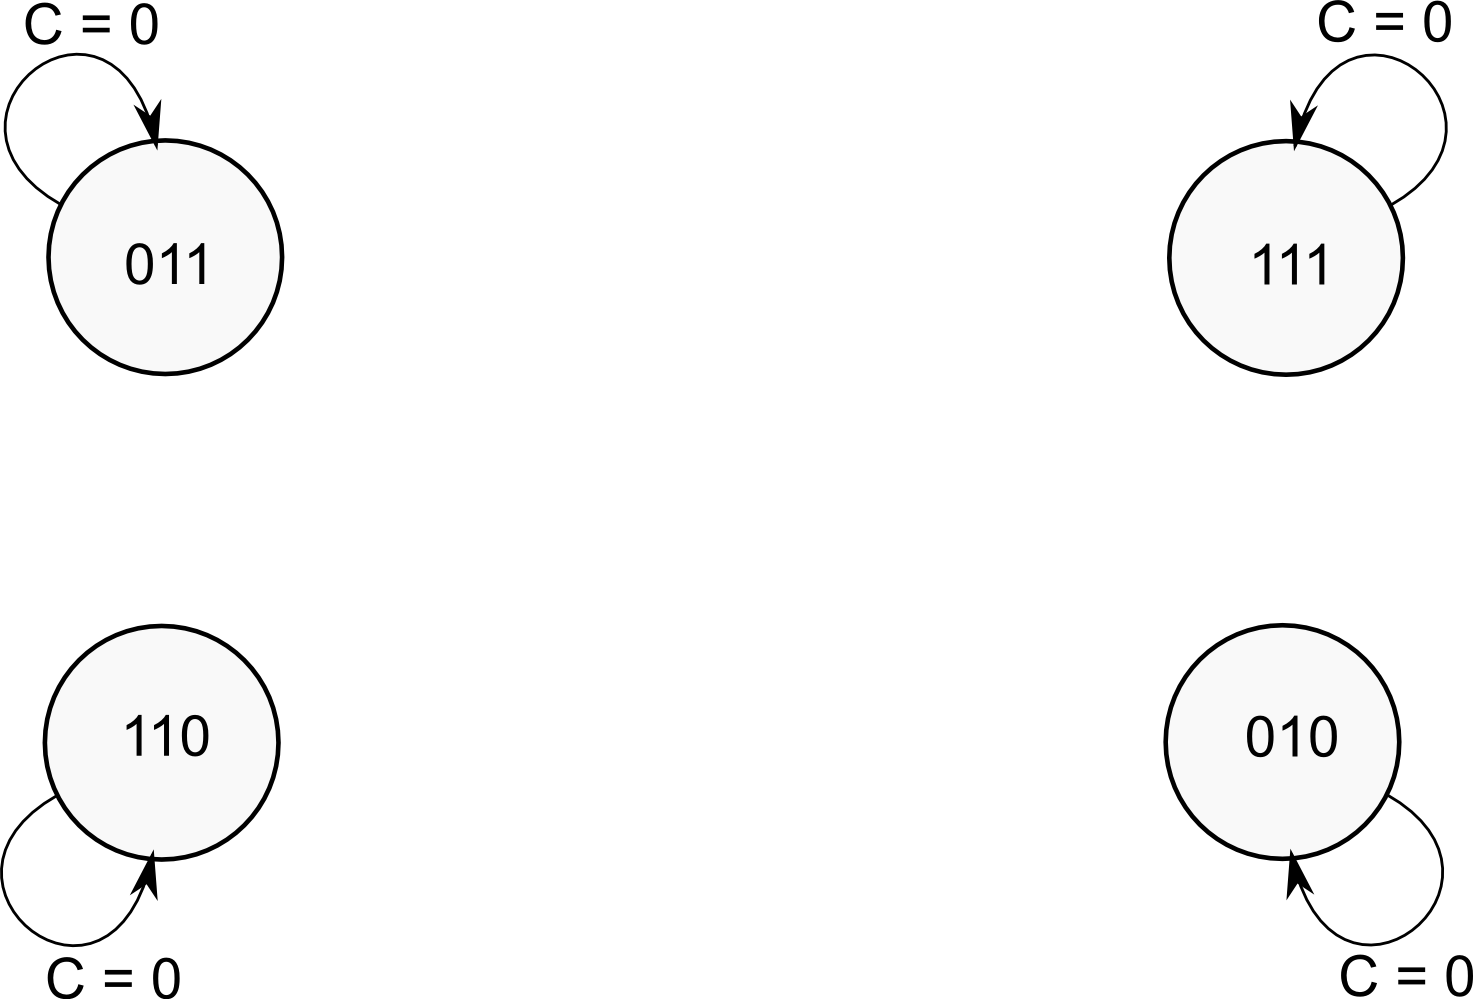
\includegraphics[height = 2.2in, width =3.5in]
      {images/exemplo_projeto_1.png}
  \end{center}
\end{frame}

\begin{frame}
  \frametitle{Exemplo(Diagrama de estados)}
  \begin{center}
    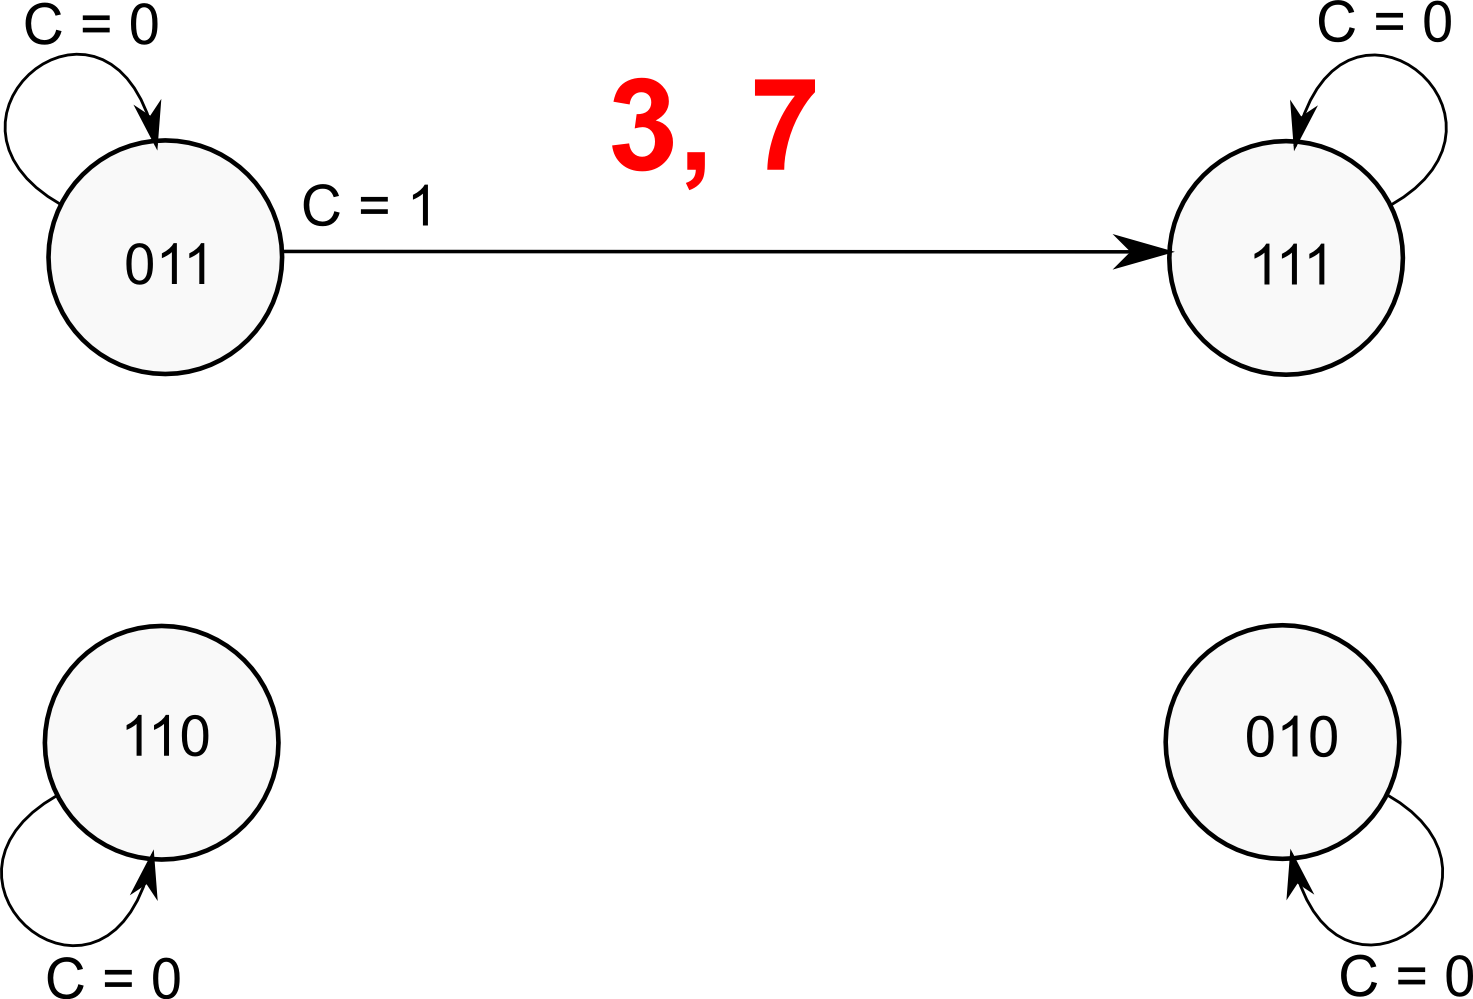
\includegraphics[height = 2.2in, width = 3.5in]
      {images/exemplo_projeto_2.png}
  \end{center}
\end{frame}

\begin{frame}
  \frametitle{Exemplo(Diagrama de estados)}
  \begin{center}
    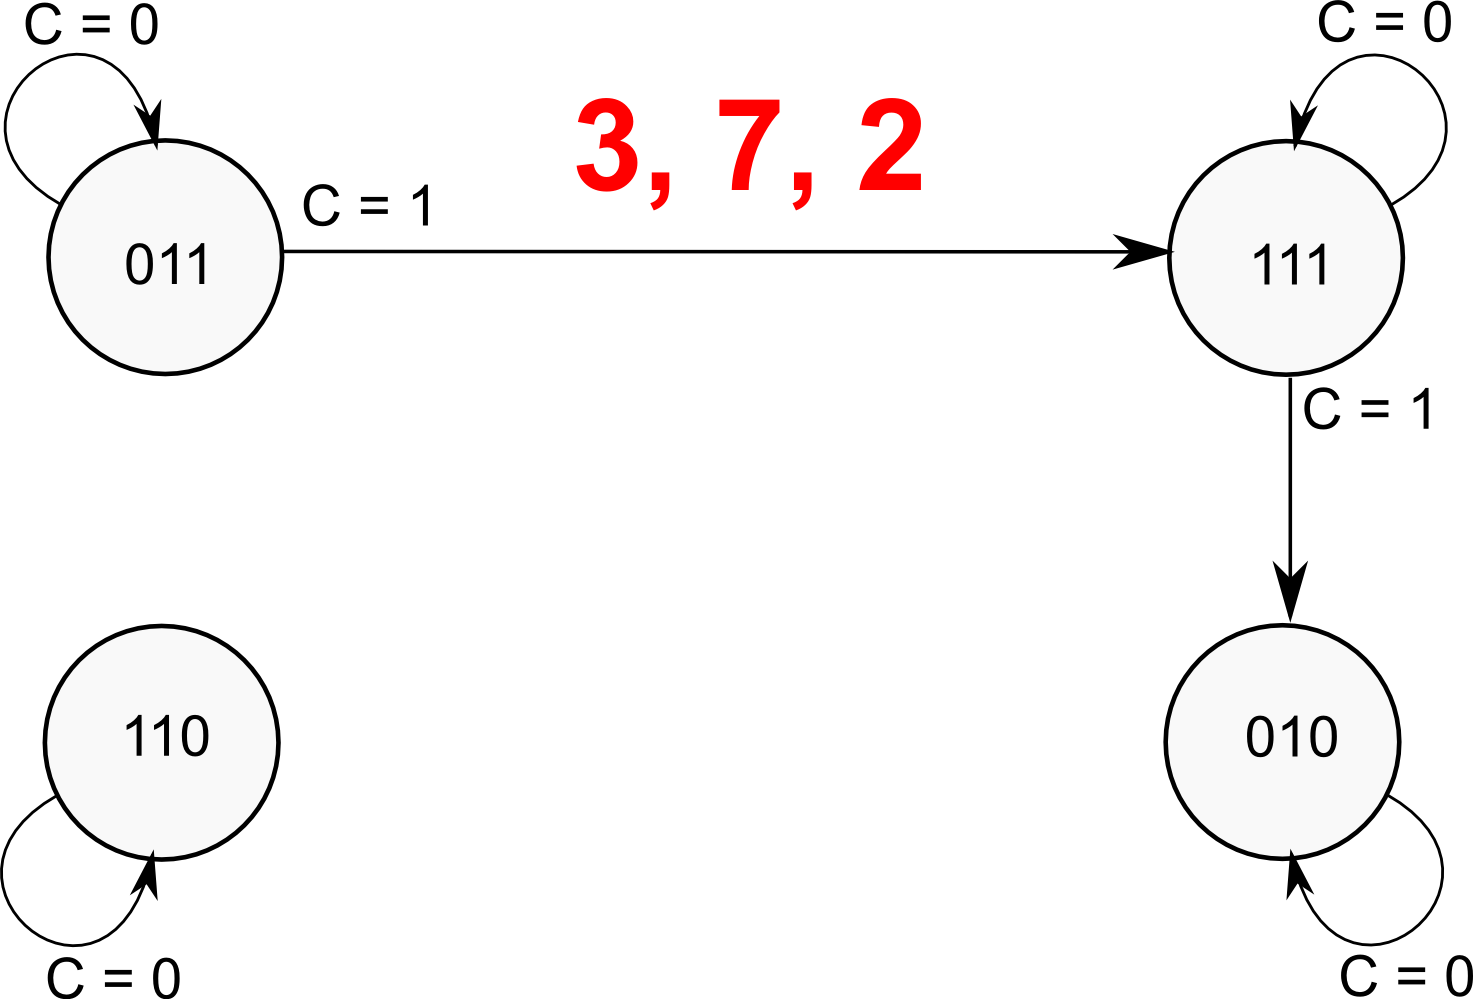
\includegraphics[height = 2.2in, width = 3.5in]
      {images/exemplo_projeto_3.png}
  \end{center}
\end{frame}

\begin{frame}
  \frametitle{Exemplo(Diagrama de estados)}
  \begin{center}
    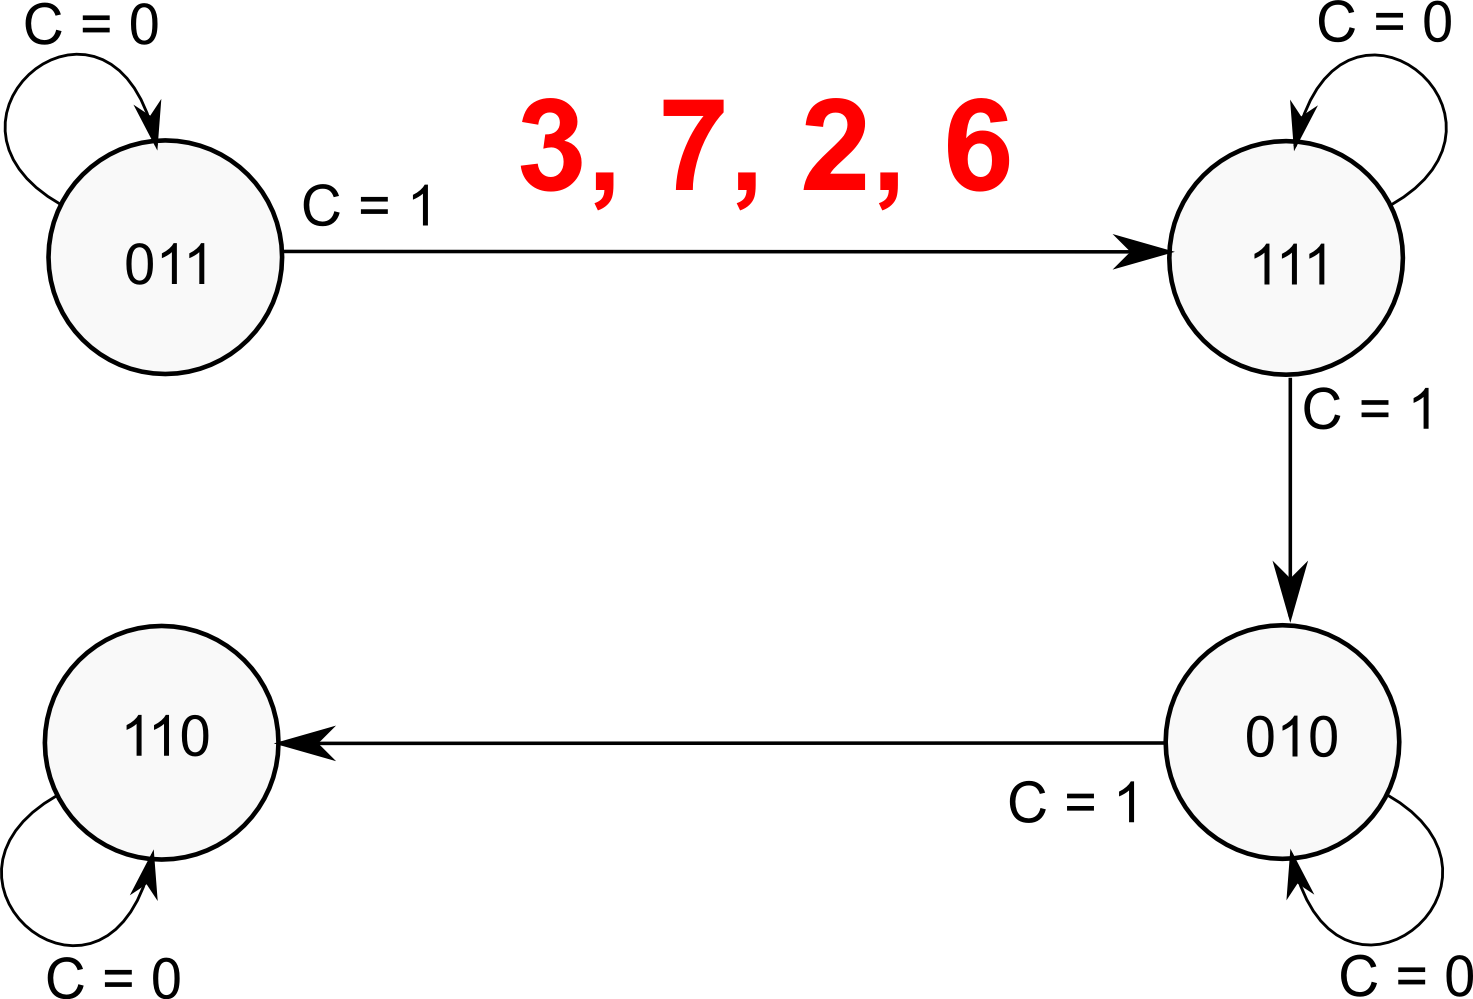
\includegraphics[height = 2.2in, width = 3.5in]
      {images/exemplo_projeto_4.png}
  \end{center}
\end{frame}

\begin{frame}
  \frametitle{Exemplo(Diagrama de estados)}
  \begin{center}
    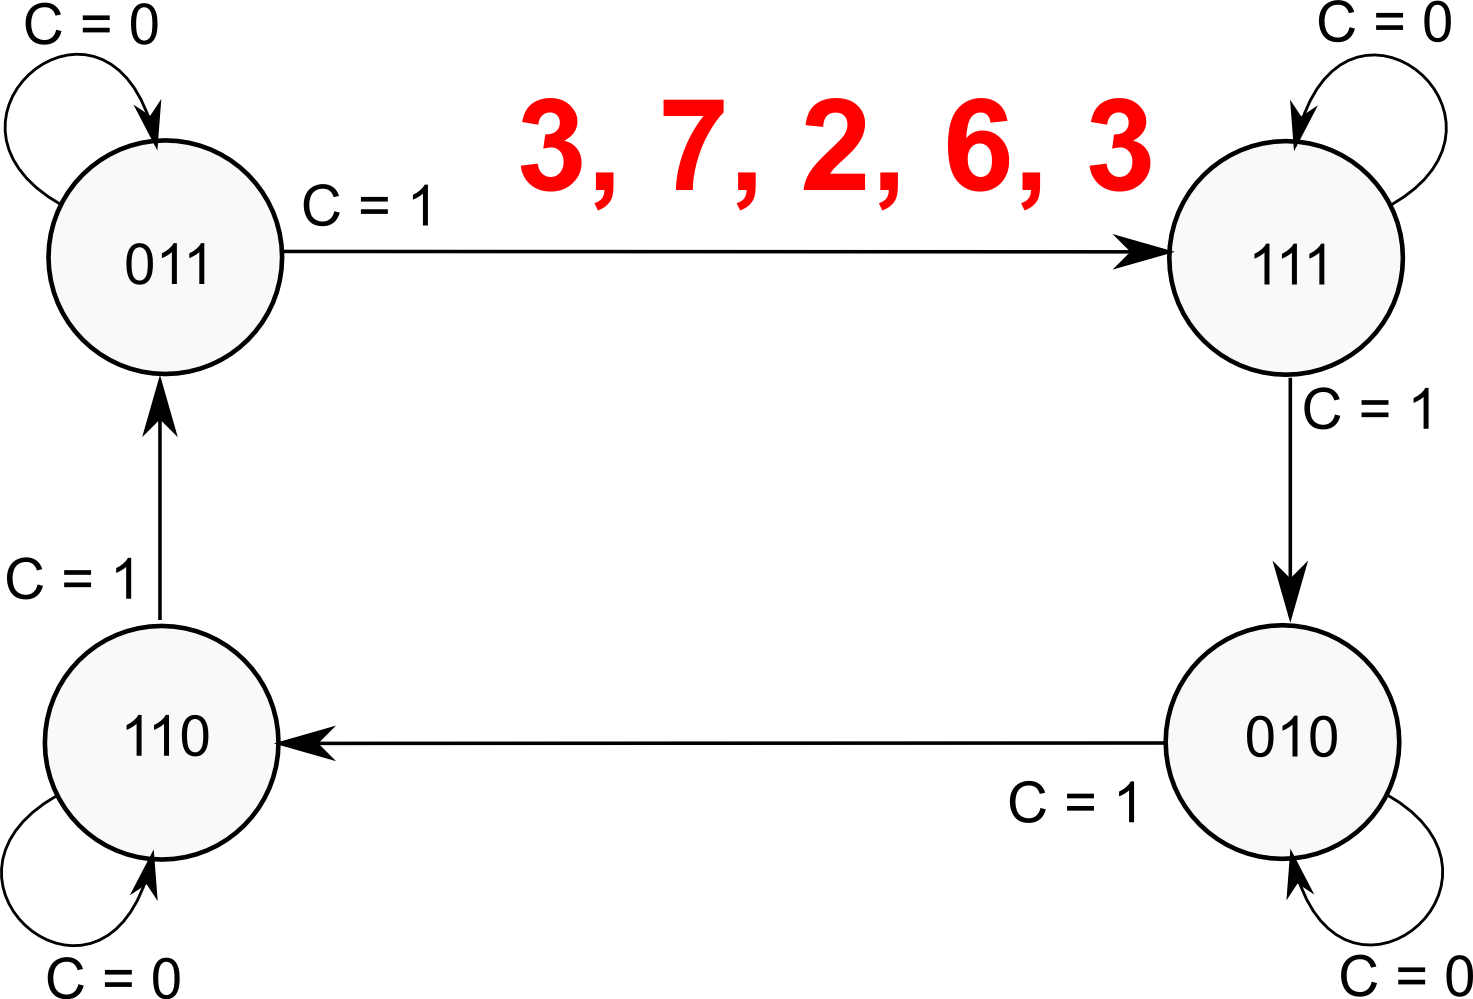
\includegraphics[height = 2.2in, width = 3.5in]
      {images/exemplo_projeto_5.png}
  \end{center}
\end{frame}

\begin{frame}
  \frametitle{Exemplo(Diagrama de estados)}
  \begin{center}
    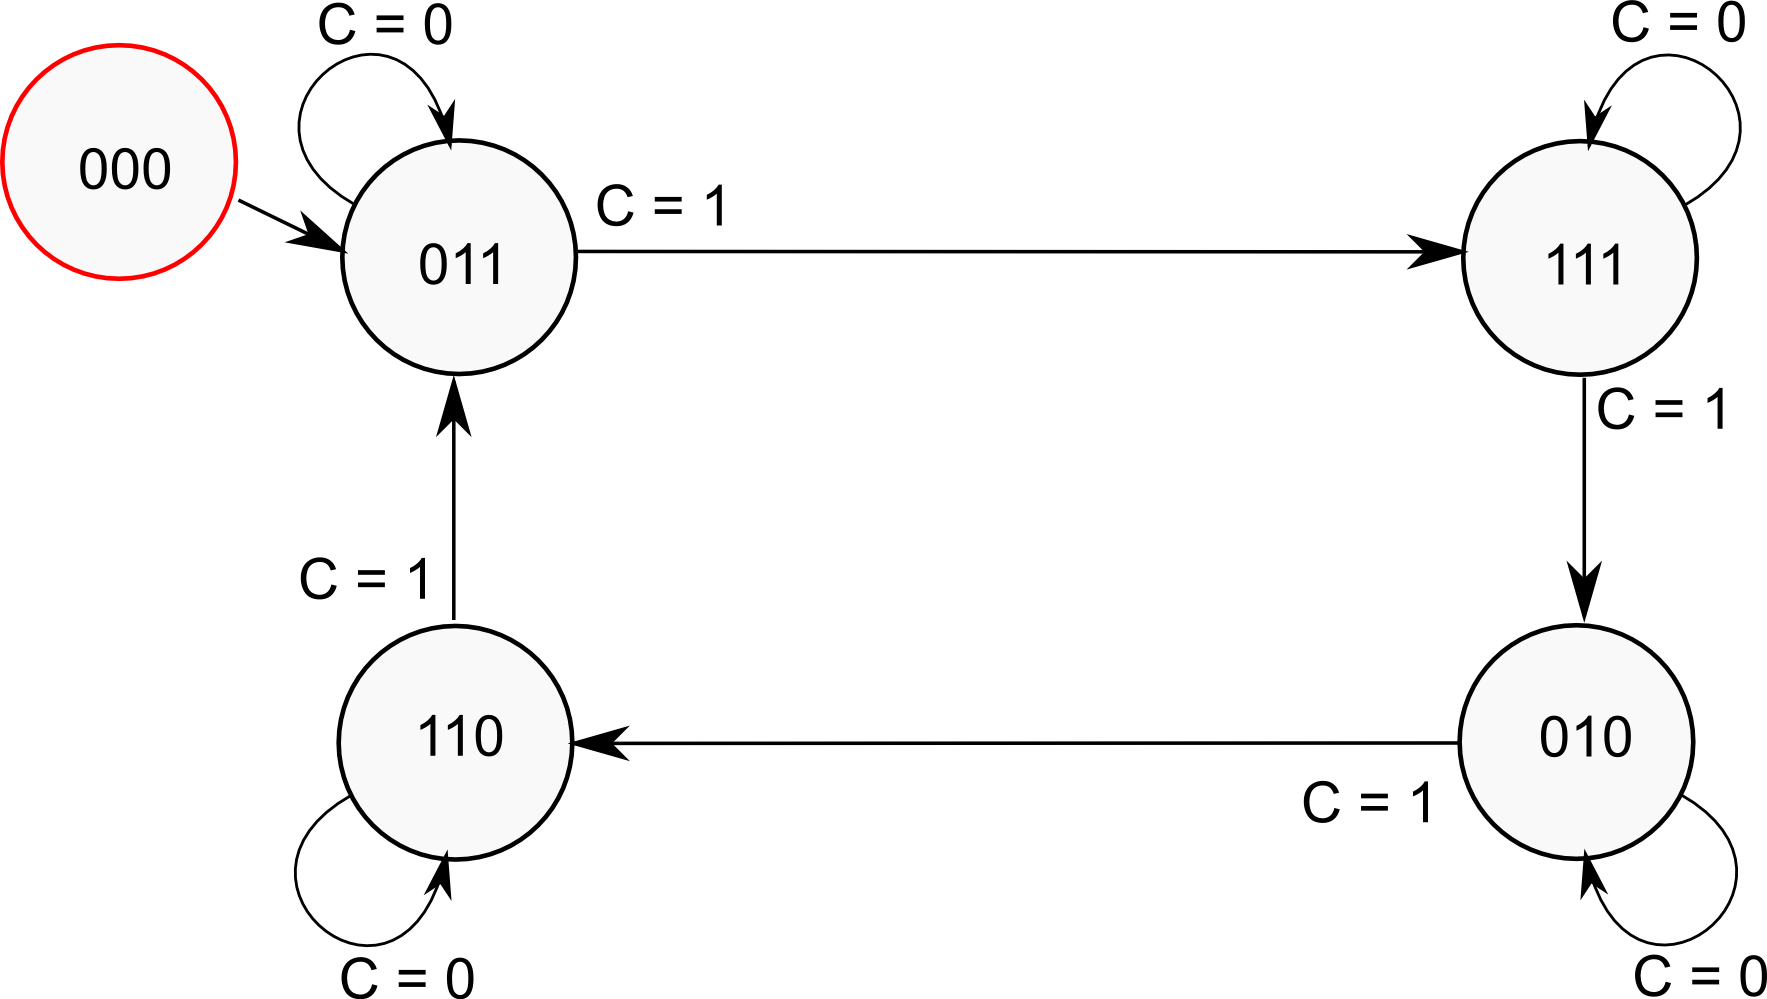
\includegraphics[height = 2.2in, width = 3.5in]
      {images/exemplo_projeto_6.png}
  \end{center}
\end{frame}

\begin{frame}
  \frametitle{Exemplo(Diagrama de estados)}
  \begin{center}
    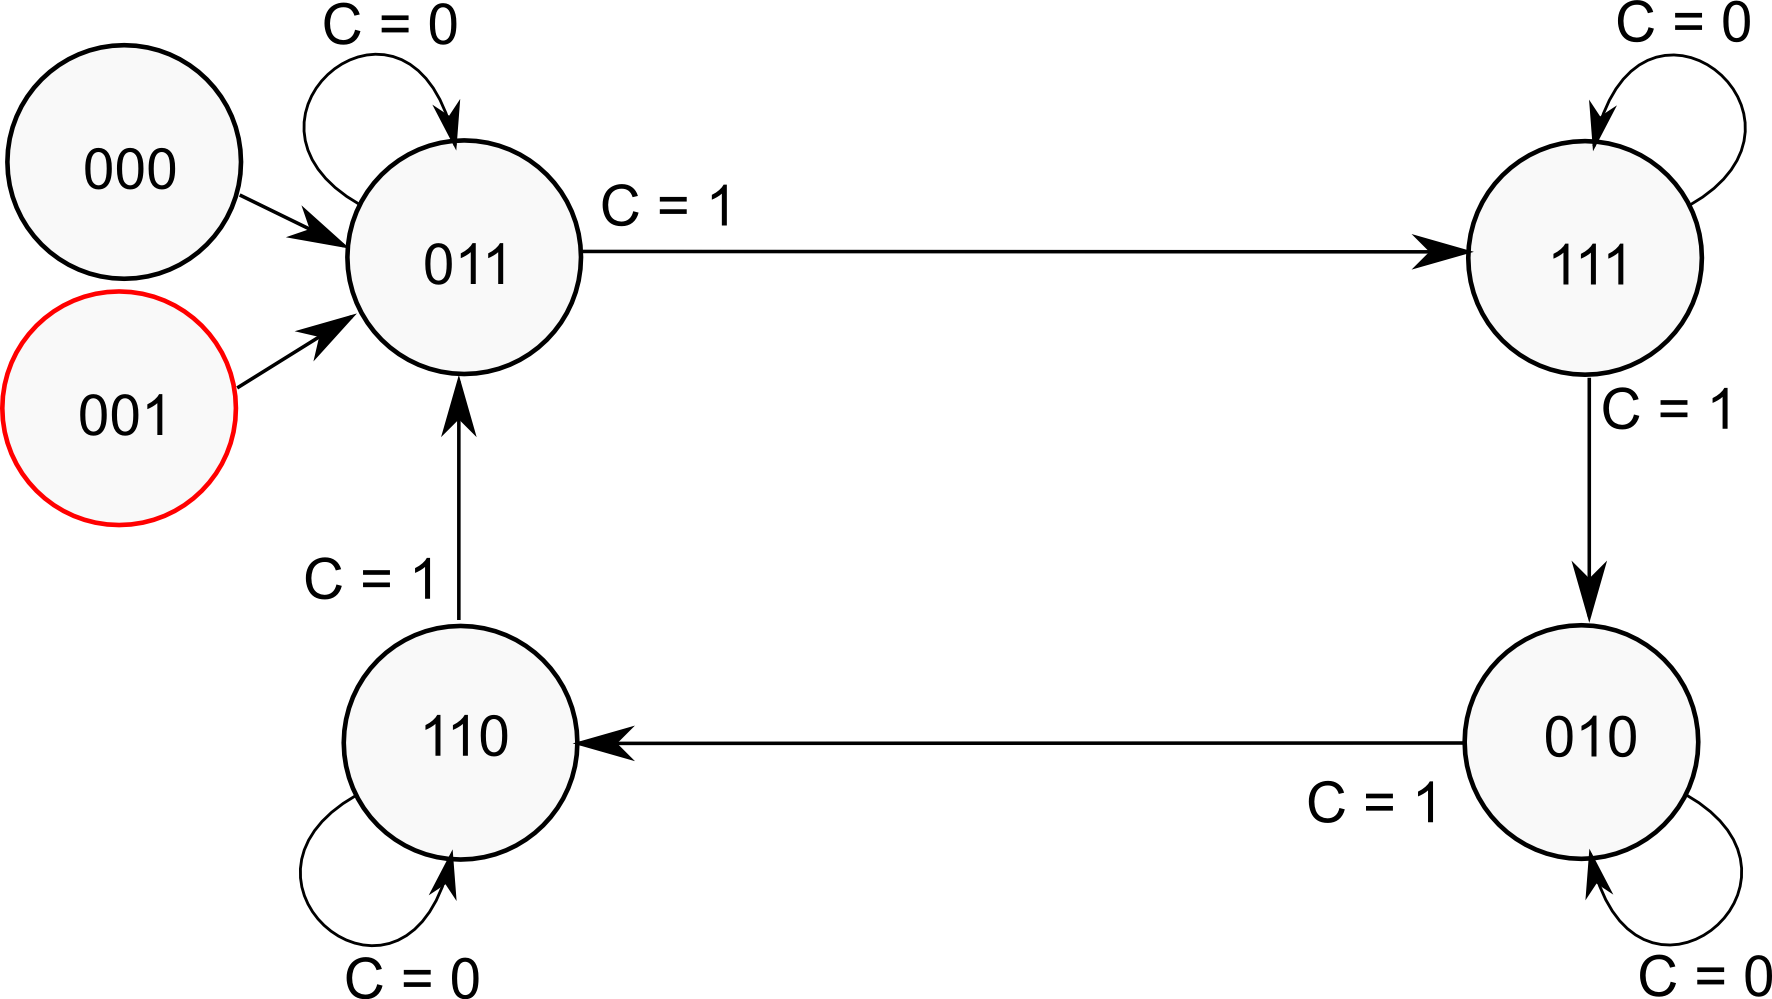
\includegraphics[height = 2.2in, width = 3.5in]
      {images/exemplo_projeto_7.png}
  \end{center}
\end{frame}

\begin{frame}
  \frametitle{Exemplo(Diagrama de estados)}
  \begin{center}
    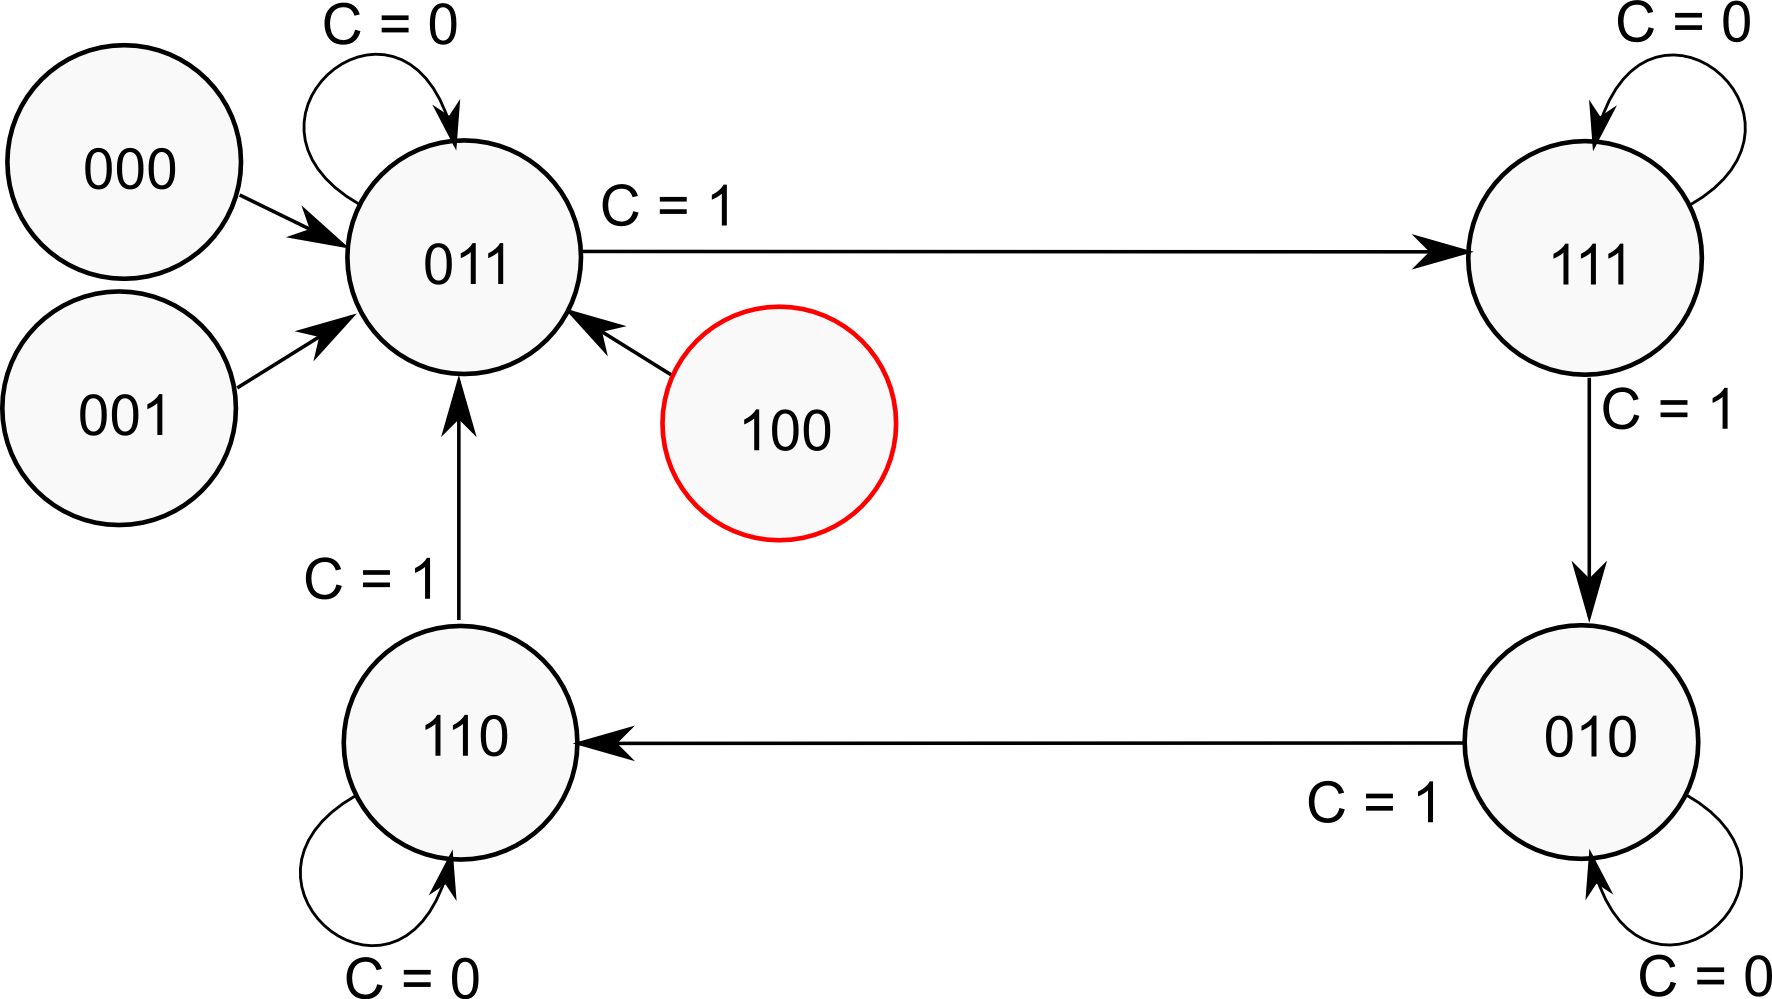
\includegraphics[height = 2.2in, width = 3.5in]
      {images/exemplo_projeto_8.png}
  \end{center}
\end{frame}

\begin{frame}
  \frametitle{Exemplo(Diagrama de estados)}
  \begin{center}
    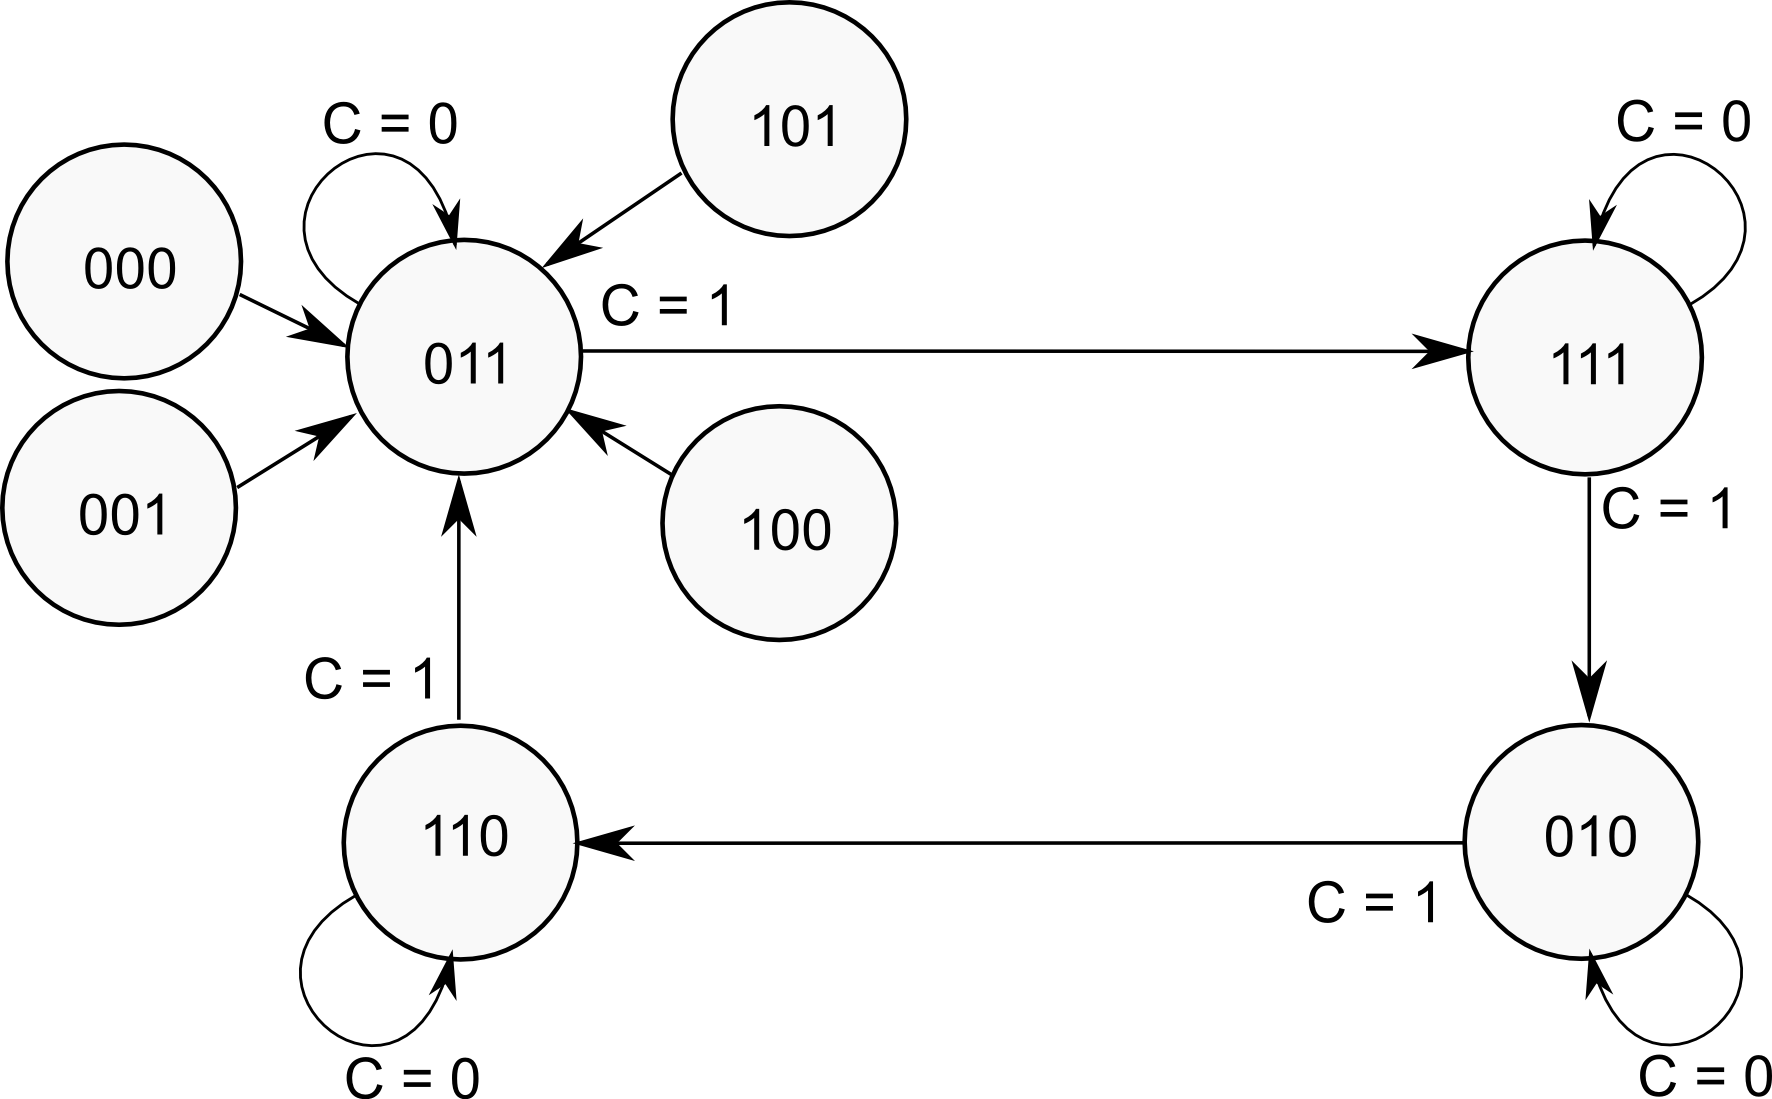
\includegraphics[height = 2.2in, width = 3.5in]
      {images/exemplo_projeto_9.png}
  \end{center}
\end{frame}

\begin{frame}
  \frametitle{Exemplo(Diagrama de estados)}
  \begin{center}
    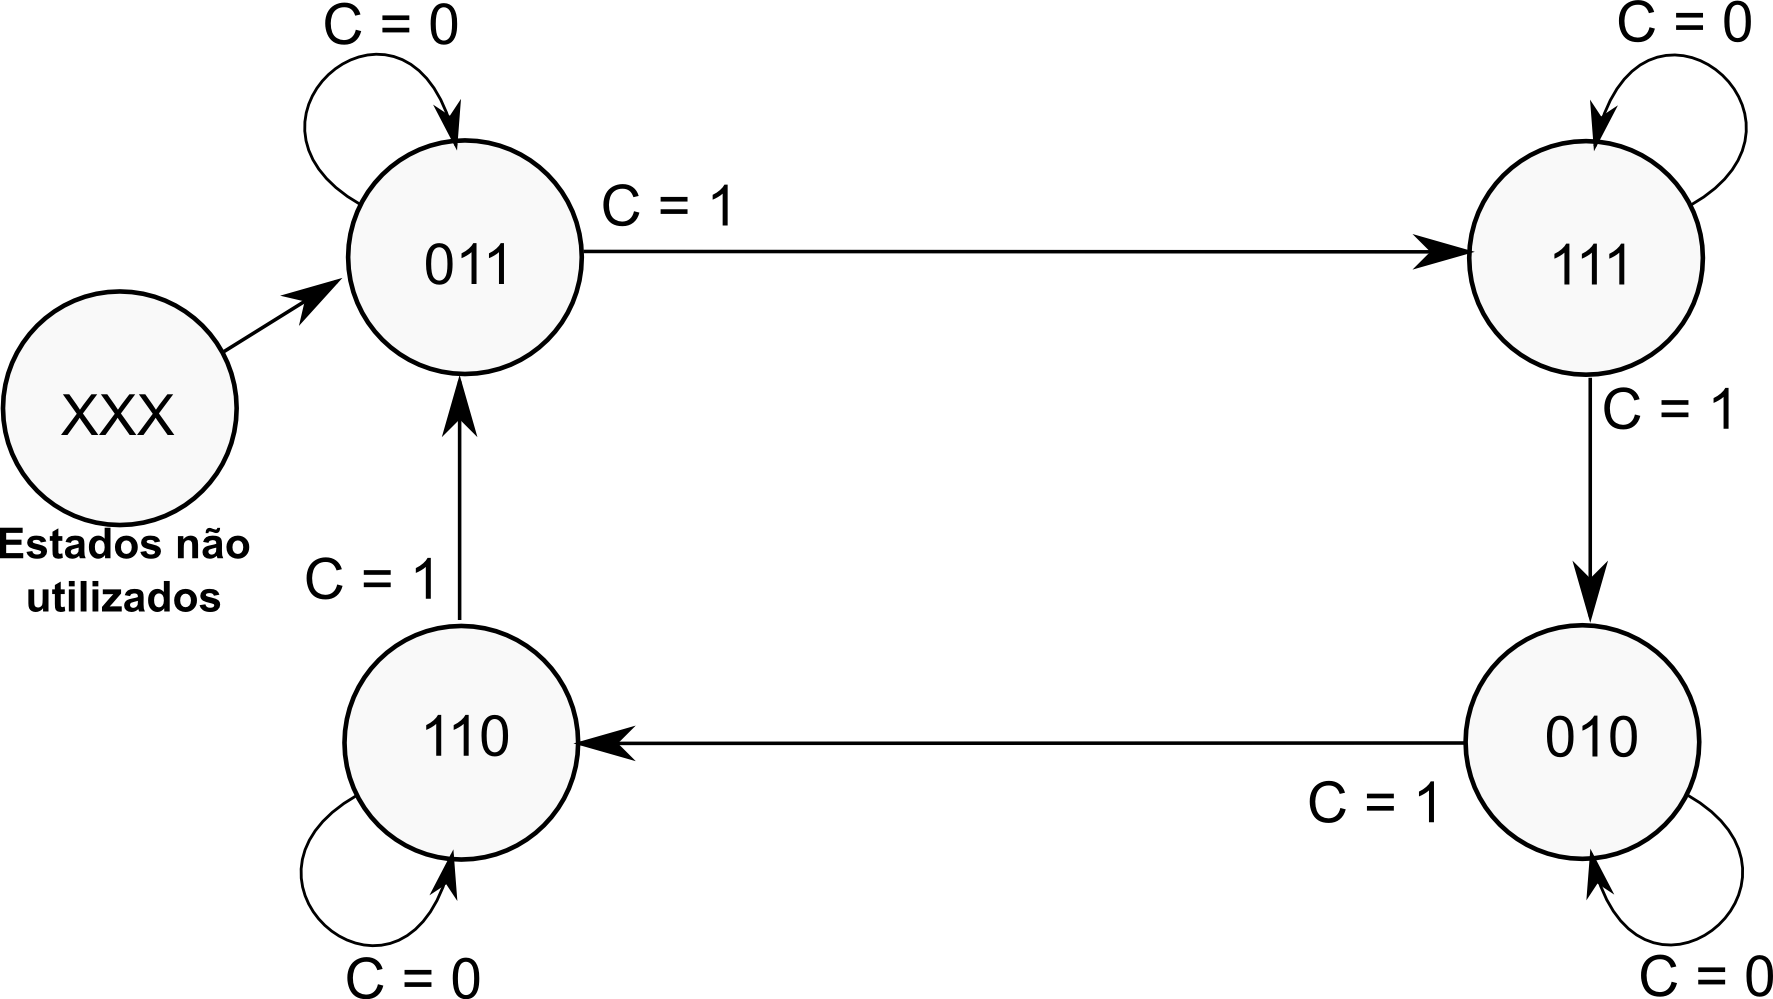
\includegraphics[height = 2.2in, width = 3.5in]
      {images/exemplo_projeto_10.png}
  \end{center}
\end{frame}


\begin{frame}
 \frametitle{Exemplo(Tabela de próximo estado)} 
  \begin{itemize}
   \item Monta-se a tabela de próximo estado com base no diagrama de estados.\pause
   \item Lembre-se que estados não utilizados são levados a 011. \pause
   \item É importante observar que esta tabela é independente do tipo de FF.\pause
   \item A tabela de próximo estado reponde a questão sobre qual será o próximo estado do FF dado o estado atual e a entrada.
  \end{itemize}
\end{frame}
  \frametitle{Exemplo(Tabela de próximo estado)} 
  
\begin{frame}
  \frametitle{Exemplo(Tabela de próximo estado)} 
  \begin{columns}[c]
   
   \begin{column}{3cm}
      \begin{center}
	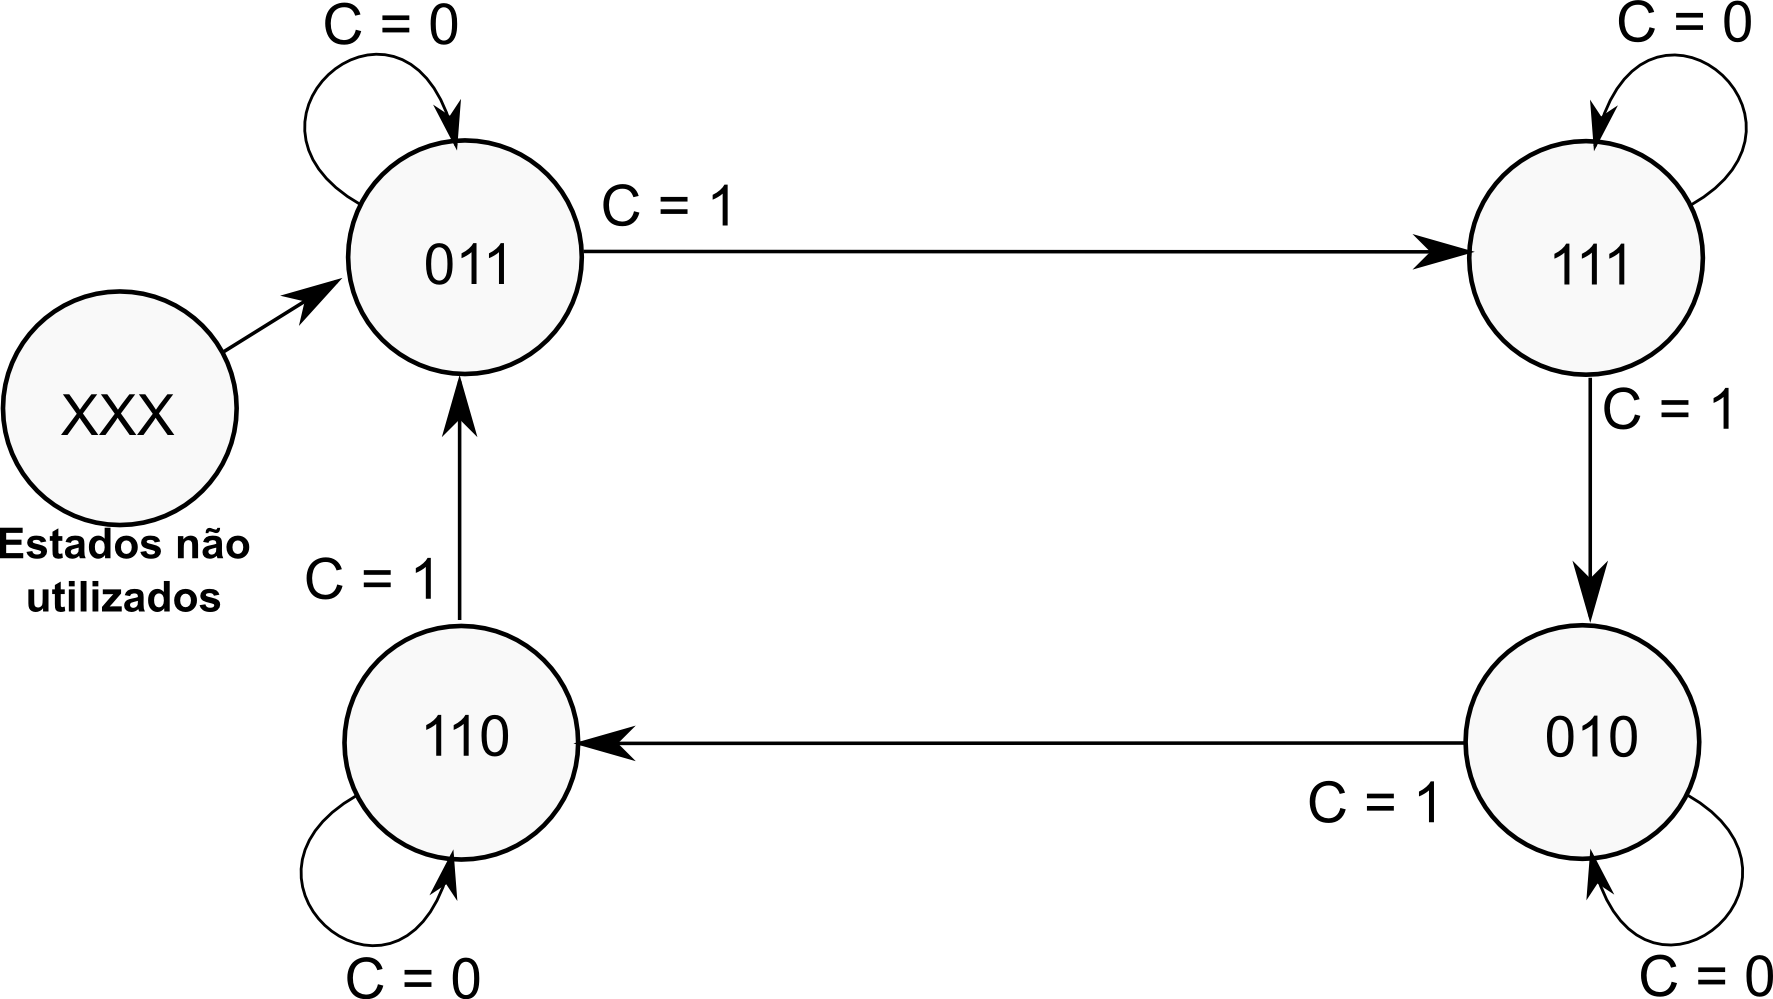
\includegraphics[height = 1in, width = 1.5in]
    {images/exemplo_projeto_10.png}
      \end{center}
   \end{column}

   \begin{column}{7cm}
       \begin{center}
	\begin{tabular}{|c|c|}
	  \hline
	    Estado atual & Próximo estado \\
	    $Q_2Q_1Q_0$  & $Q_{2next}Q_{1next}Q_{0next}$ \\
			 & \begin{tabular}{c|c} C = 0 & C = 1 \\ \end{tabular} \\
	  \hline
	    000 \pause & \begin{tabular}{c|c} 011 \pause & 011 \pause\\ \end{tabular} \\
	  \hline
	    001 \pause & \begin{tabular}{c|c} 011 \pause & 011 \pause\\ \end{tabular} \\
	  \hline
	    010 \pause & \begin{tabular}{c|c} 010 \pause & 110 \pause\\ \end{tabular} \\
	  \hline
	    011 \pause & \begin{tabular}{c|c} 011 \pause & 111 \pause\\ \end{tabular} \\
	  \hline
	    100 \pause & \begin{tabular}{c|c} 011 \pause & 011 \pause\\ \end{tabular} \\
	  \hline
	    101 \pause & \begin{tabular}{c|c} 011 \pause & 011 \pause\\ \end{tabular} \\
	  \hline
	    110 \pause & \begin{tabular}{c|c} 110 \pause & 011 \pause\\ \end{tabular} \\
	  \hline
	    111 \pause & \begin{tabular}{c|c} 111 \pause & 010 \pause\\ \end{tabular} \\
	  \hline
	\end{tabular}
      \end{center}
   \end{column}
  \end{columns}
\end{frame}

\begin{frame}
 \frametitle{Exemplo(Tabela de implementação)} 
  \begin{itemize}
   \item Esta tabela é construída com base na tabela do próximo estado e \emph{por meio das tabelas especificas de cada FF.}\pause
   \item O FF D é o único FF no qual a tabela de implementação é igual a tabela de próximo estado.
  \end{itemize}
\end{frame}

\begin{frame}
 \frametitle{Exemplo(Tabela de implementação)} 
 \begin{center}
	\begin{tabular}{|c|c|}
	  \hline
	    Estado atual & Próximo estado \\
	    $Q_2Q_1Q_0$  & $D_{2next}D_{1next}D_{0next}$ \\
			 & \begin{tabular}{c|c} C = 0 & C = 1 \\ \end{tabular} \\
	  \hline
	    000  & \begin{tabular}{c|c} 011  & 011 \\ \end{tabular} \\
	  \hline
	    001  & \begin{tabular}{c|c} 011  & 011 \\ \end{tabular} \\
	  \hline
	    010  & \begin{tabular}{c|c} 010  & 110 \\ \end{tabular} \\
	  \hline
	    011  & \begin{tabular}{c|c} 011  & 111 \\ \end{tabular} \\
	  \hline
	    100  & \begin{tabular}{c|c} 011  & 011 \\ \end{tabular} \\
	  \hline
	    101  & \begin{tabular}{c|c} 011  & 011 \\ \end{tabular} \\
	  \hline
	    110  & \begin{tabular}{c|c} 110  & 011 \\ \end{tabular} \\
	  \hline
	    111  & \begin{tabular}{c|c} 111  & 010 \\ \end{tabular} \\
	  \hline
	\end{tabular}
      \end{center} 
\end{frame}

\begin{frame}
 \frametitle{Exemplo(Equações de excitação)} 
  \begin{itemize}
   \item Para cada entrada do FF deve haver uma equação de excitação.\pause
   \item As equações de excitação são o que causam a mudança de estado na memória.
  \end{itemize}
\end{frame}

\begin{frame}
 \frametitle{Exemplo(Equações de excitação)} 
      \begin{center}
	\begin{tabular}{|c|c|}
	  \hline
	    Estado atual & Próximo estado \\
	    $Q_2Q_1Q_0$  & $D_{2next}D_{1next}D_{0next}$ \\
			 & \begin{tabular}{c|c} C = 0 & C = 1 \\ \end{tabular} \\
	  \hline
	    000  & \begin{tabular}{c|c} \textbf{0}11  & \textbf{0}11 \\ \end{tabular} \\
	  \hline
	    001  & \begin{tabular}{c|c} \textbf{0}11  & \textbf{0}11 \\ \end{tabular} \\
	  \hline
	    010  & \begin{tabular}{c|c} \textbf{0}10  & \textbf{1}10 \\ \end{tabular} \\
	  \hline
	    011  & \begin{tabular}{c|c} \textbf{0}11  & \textbf{1}11 \\ \end{tabular} \\
	  \hline
	    100  & \begin{tabular}{c|c} \textbf{0}11  & \textbf{0}11 \\ \end{tabular} \\
	  \hline
	    101  & \begin{tabular}{c|c} \textbf{0}11  & \textbf{0}11 \\ \end{tabular} \\
	  \hline
	    110  & \begin{tabular}{c|c} \textbf{1}10  & \textbf{0}11 \\ \end{tabular} \\
	  \hline
	    111  & \begin{tabular}{c|c} \textbf{1}11  & \textbf{0}10 \\ \end{tabular} \\
	  \hline
	\end{tabular}
      \end{center} 
      $D_2 = Q_2Q_1\overline{C} + \overline{Q_2}Q_1C$ 
\end{frame}

\begin{frame}
 \frametitle{Exemplo(Equações de excitação)} 
     $D_2 = Q_2Q_1\overline{C} + \overline{Q_2}Q_1C$  \\
     $D_1 = 1$ \\
     $D_2 = \overline{Q_1} + \overline{Q_2}Q_0 + Q_0\overline{Q_C} + Q_2\overline{Q_0}C$
\end{frame}

%SEÇÃO == BIBLIOGRAFIA
\section{Bibliografia}
\begin{frame}
 \frametitle{Referências bibliográficas}
 \begin{itemize}
  \item Digital Logic and Microprocessor Design With VHDL – Enoch O . Hwang
  \item Digital Design Principles And Practices - Wakerly
 \end{itemize}
\end{frame}

\end{document}
